\documentclass[UTF8]{ctexart}
\usepackage{booktabs}  % professionally typeset tables
\usepackage{amsmath}
\usepackage{setspace}
\usepackage{textcomp}  % better copyright sign, among other things
\usepackage{xcolor}
\usepackage{lipsum}    % filler text
%\usepackage{subfig}
\usepackage{geometry}
\usepackage{float}
\usepackage{hyperref}
\usepackage{graphicx}


%\geometry{left=2.54cm,right=2.54cm,top=2.18cm,bottom=3.18cm}
\date{}
\title{\textbf{通信原理实验}}
\author{无45 \ *** \ **********\\
        无45 \ 孙径舟 \ 2014011153\\
        无46 \ 黄秀峰 \ 2014011193\\
        无47 \ 刘畅 \ 2014011196}


\begin{document}
\maketitle

\section{实验目的}

\begin{itemize}

\item 根据所学习的现代通信原理知识,自己设计实验题目,并根据题目的需要在实验平台上选用所需要的器件,完成设计;
\item 提高对现代通信原理中一些基础理论的理解和运用;
\item 锻炼自学能力,提高设计能力,培养团队精神。

\end{itemize}

\section{实验平台}

实验平台主要包括以下几部分:FPGA(FLEX10K30RC240)、FLASH、锁相环、压控振荡器、单片机、直接数字频率综合器、码型变换、存储器、带低通滤波器的模数转换、带低通滤波器的数模转换、拨码开关、晶体振荡器和二极管显示等部分。我们主要使用了:FPGA、D/A转换器、拨码开关和晶体振荡器。

\section{实验内容}

设计一个包含信道编解码、交织、调制解调等模块的通信系统,并前其在FPGA平台上实现

\subsection{系统功能}

系统包含信道编解码、交织、调制解调等模块,可实现比特流的传输

\subsection{系统结构}

系统按顺序包括如下模块:

\begin{itemize}

\item 信道编码
\item 交织
\item 调制
\item 信道模拟
\item 解调
\item 解交织
\item 信道解码

\end{itemize}



\subsubsection{信道编码模块}
卷积码将k个信息比特编码成n个比特,适合以串行形式传。其编码器一般表示为$(n,k,m)$的形式,其中k为每次输入到卷积编码器的比特数,n为每次输入k位比特后输出的编码长度,m为编码存储长度。

本次实验中,我们使用的是$(2,1,3)$卷积编码,每输入一个信息比特,编码产生两位比特的输出,其框图如图.\ref{fig:encoder}所示。

\begin{figure}[htb]
\centering
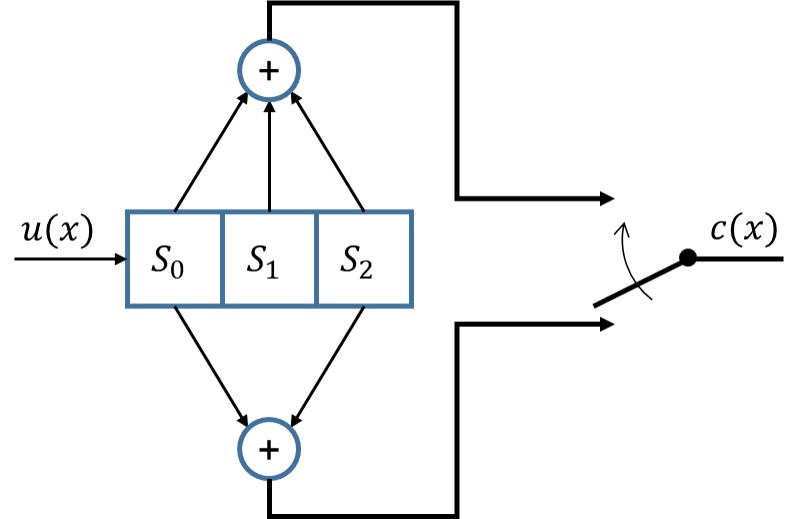
\includegraphics[width=0.4\textwidth]{images//encoder.jpg}
\caption{\label{fig:encoder}(2,1,3)编码器}
\end{figure}

编码器的输入端口信号为:
\begin{itemize}
\item clk\quad        输入控制时钟
\item clk2\quad       输出控制时钟
\item data\_in\quad    编码数据输入
\item reset\quad    重置位
\end{itemize}
其中clk2用于对编码后数据进行控制输出,由于我们采用$(2,1,3)$编码器,故而clk2的频率是clk的两倍。

编码器的输出端口信号为:
\begin{itemize}
\item code\_out\quad        编码数据输出
\item valid\quad       编码有效标志位
\item valid\_wave\quad    编码有效信息流
\end{itemize}
由于我们设计了交织和调制解调模块,需要保证信号同步才能使系统正确工作,所以我们设计了valid以及valid\_wave这两个控制信号来进行各模块间的信号同步。

我们还定义了一个寄存器数组state,用于存储之前时刻的输入。由框图可知,code\_out和state的关系可以表示为:\\
\quad\quad\quad code\_out[0]~=~data\_in + state[0] + state[1]\\
\quad\quad\quad code\_out[1]~=~data\_in + state[1]

每次输入一位比特,编码两位输出,并将valid置为有效。当reset有效时,state清空,并将valid置为无效。

仿真波形如图.\ref{fig:fangzhen}所示。其中data\_send为原始序列,code\_send为编码后序列;二者对应的时钟分别为clk\_div2和clk。从图中可以看出,data\_send每字符占用周期是code\_send两倍。下面用Python检验了一下输出结果,如图
.\ref{fig:PythonSimu},可见我们的编码是正确的。

\begin{figure}[htb]
\centering

\includegraphics[width=0.9\textwidth]{images//encoder_simulation.jpg}
\caption{\label{fig:fangzhen}(2,1,3)编码器仿真波形}
\end{figure}

\begin{figure}[htb]
\centering
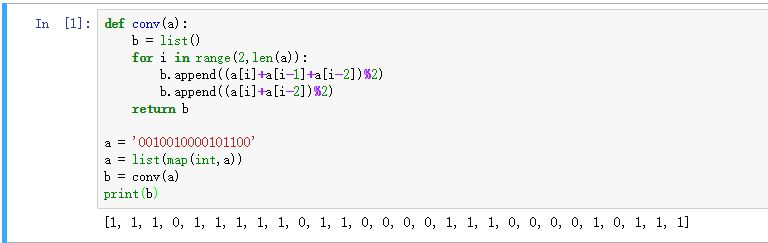
\includegraphics[width=0.8\textwidth]{images//python_simulation.jpg}
\caption{\label{fig:PythonSimu}(2,1,3)编码器输出}
\end{figure}



\subsubsection{交织模块}

\paragraph{交织器的原理及作用}

在通信中,传输信息比特差错经常是成串发生的。然而,信道编码仅在检测和校正单个差错和不太长的差错串时才有效。为了解决这一问题,希望能找到把一条消息中的相继比特分散开的方法,即一条消息中的相继比特以非相继方式被发送。这样,在传输过程中即使发生了成串差错,恢复成一条相继比特串的消息时,差错也就变成单个(或长度很短),这时再用信道编码纠错功能纠正差错,恢复原消息。简单来说,交织就是将信道传输过程中的连续差错分散化。

\paragraph{交织器的实现}

本实验中采用最常见的交织方法——行列交织。行列交织基本的原理如下图所示:

\begin{figure}[H]
    \centering
    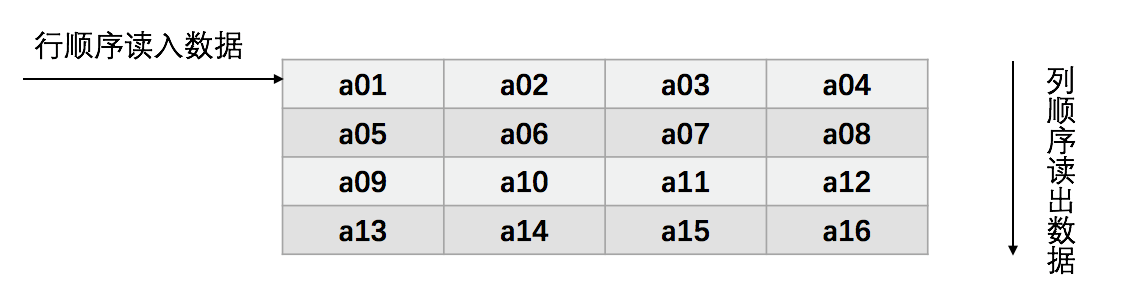
\includegraphics[width=\textwidth]{images//inter_input.png}
\end{figure}

即行顺序写入寄存器,列顺序读出。上图交织结果为a01,a05,a09,a13,a02,a06,a10,a14,a03,a07,a11,a15,a04,a08,a12,a16


本实验中实现行列交织的具体算法为:

使用两个寄存器数组,一个的作用为行顺序接收当前输入数据并存储时另一个负责按照列顺序输出数组中存储数据。每周期读入一个比特,每16个周期两数组作用互换。

每一周期读入比特的流程图如下:

\begin{figure}[H]
    \centering
    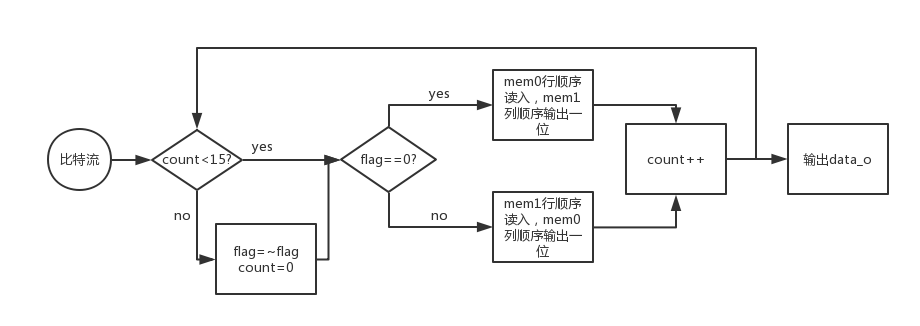
\includegraphics[width=\textwidth]{images//inter_pic.png}
\end{figure}

初始时:count=0;flag=0;mem0[15:0],mem1[15:0]=0;data\_o=0;

\newpage


\subsubsection{调制模块}

\subsubsection{信道模拟模块}

\subsubsection{解调模块}

\subsubsection{解交织模块}

解交织模块与交织模块相同

\subsubsection{信道解码模块}
信道解码使用维特比译码器,判决方式为硬判决。设计思路如下:

\paragraph{变量设计}

\begin{itemize}
\item \textbf{codebuff} : 接收的码流,存于缓冲区中,数量达到一组后送入译码区
\item \textbf{code} : 译码区码流,即当然需要译码的码流
\item \textbf{possible\_codex} : 维特比译码图中,当前阶段第x个状态(共有四个状态)所对应的最优路径
\item \textbf{errorx} : 第x个最优路径(共有4 条路径)对应的判决误差
\item \textbf{decodex} : 维特比译码中,当前阶段第x状态的最优路径所对应的输出译码
\item \textbf{decode} : 前一组码流(已译码结束)所对应的输出译码
\end{itemize}

\paragraph{译码流程}

\begin{enumerate}
\item 接收码流至codebuff,当接收完一组后,送入code中等待译码
\item 每一个时钟周期,译码往前推进两位,求出当前状态下的最优路径并计算硬判决误差,并记录四个状态所对应的最优路径
\item 完成一组译码后,将译码结果存入decode,之后每一个时钟周期输出一位译码结果
\end{enumerate}

\subsection{软件仿真}
软件仿真具体情况如下:

\begin{itemize}
\item 仿真平台:ModelSim-Altera 10.4b
\item 输入序列:[1, 0, 0, 1, 0, 0, 0, 0, 1, 0, 1, 1, 0, 0]
\item 编码方式:(2,1,3)卷积码
\item 调制方式:QPSK
\item 是否交织:是
\item 是否加噪声:是
\end{itemize}

编码输入及输出波形已在原理部分有所展示,在此不予赘述。我们将考虑的内容包括:(1)通过噪声信道前后发送序列;(2)编码后序列与解码输入;(3)解码后序列与原始序列。\\

\noindent {\bf \large 通过噪声信道前后发送序列}

通过噪声信道前序列即交织后序列,记作bit\_send。而通过噪声信道后的序列记作bit\_recv。如.\ref{fig:BitSig} 中所示,由于交织需要一定的缓冲,从而两个信号之间存在延迟。仔细观察可以看出,这两个序列存在一些差异,这是由于我们添加的噪声较大,正好用来检验卷积码的纠错能力。
\begin{figure}[htb]
\centering
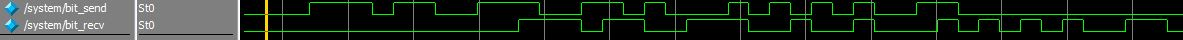
\includegraphics[width=1.2\textwidth]{images//BitSig.jpg}
\caption{\label{fig:BitSig}通过噪声信道前后序列}
\end{figure}\\

\noindent {\bf \large 编码后序列与解码输入}

编码后序列及code\_send,而解码输入记作code\_recv,分别如图.\ref{fig:CodeSend},图.\ref{fig:CodeRecv}所示。同样的,由于信道噪声较强,二者并不一样。
\begin{figure}[htb]
\centering
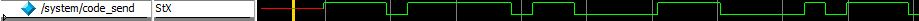
\includegraphics[width=1.2\textwidth]{images//CodeSend.jpg}
\caption{\label{fig:CodeSend}编码后序列}
\end{figure}
\begin{figure}[htb]
\centering
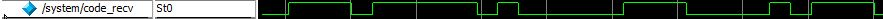
\includegraphics[width=1.2\textwidth]{images//CodeRecv.jpg}
\caption{\label{fig:CodeRecv}解码输入序列}
\end{figure}\\

\noindent {\bf \large 解码后序列与原始序列}

解码后序列记为data\_recv, 如图.\ref{fig:DataRecv}所示,和输入序列完全相同,体现了卷积码的纠错能力。
\begin{figure}[htb]
\centering

\includegraphics[width=1.2\textwidth]{images//DataRecv.jpg}
\caption{\label{fig:DataRecv}解码后序列}
\end{figure}
我们还可以观察一下Viterbi算法给出的最大似然输入,记作code\_prob,如如图.\ref{fig:CodeProb}所示,和code\_send完全相同。
\begin{figure}[htb]
\centering
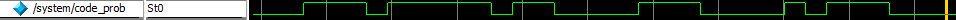
\includegraphics[width=1.2\textwidth]{images//CodeProb.jpg}
\caption{\label{fig:CodeProb}最大似然输入}
\end{figure}

单独看起来,每个模块都不算复杂,无非是对输入数据做一些处理。但当我们试图把这些模块组合成一个系统是,同步成了最为关键的问题。举例来说,对于交织模块,如果我们交织的部分和实际输入存在1bit偏差,这样相当于在编码后结果前加一位0,并减去末尾一比特。这对于卷积码来说是灾难性的错误,我们将不可能恢复出正确的序列。
为了解决同步的问题,我们为每个模块都设置了同步信号。只有当下一级模块收到上一级模块的有效同步信号时,才开始进行相关的操作。牺牲一部分延时性能来换取同步的准确性。



\section{实验总结}
在本次实验中,我们设计了基于(2,1,3)卷积码和QPKS调制的通信系统,使用LED灯作为输出,在有噪声的情况下检验了该系统的性能。实验证明,卷积码在一定噪声情况下依然可以有较好的性能。

由于我们对于卷积码有着较为充分的了解,且团队成员中有人非常擅长编写Verilog程序,因此总体上实验进行的较为顺利。虽然如此,各模块之间的同步依然是一个比较困扰我们的问题。在最开始设计的时候我们没有充分考虑到模块同步性的问题,仿真中出现了颇令人费解的现象,在逐级排查解决问题之后,我们终于使得系统能够正常工作。不过此时在边界情况下仍然存在一些小问题,我们尝试了不同的输入情况,尽可能充分地解决了这些问题。

最后,感谢老师和助教们这一学期的悉心指导和辛苦付出,祝二零一八年一切顺利!\\




{\bf \Large 分工情况:}
\begin{itemize}
\item 黄天昊:信道调制解调/噪声模块编写,以及相应部分报告撰写。
\item 孙径舟:卷积编码,模块联调与测试,以及相应部分报告撰写。{\bf 软件仿真}与{\bf 总结}撰写。
\item 黄秀峰:卷积解码,模块联调与测试,以及相应部分报告撰写。{\bf 实验情况介绍}撰写。
\item 刘畅:交织/解交织模块编写,以及相应部分报告撰写。
\end{itemize}



\end{document}










